%! TEX root = ../main.tex
\documentclass[../main.tex]{subfiles}
\begin{document}
\section{Einführung in den 3D-Druck}
Der 3D-Druck, auch bekannt als \acrfull{am} oder \gls{rp} ist ein bereits länger bekanntes Forschungs- und Entwicklungsfeld, da bereits im Jahr 1986 das erste Verfahren, \acrfull{sla} von Charles Hull entwickelt wurde.
Ein moderner Drucker dieses Verfahrens ist in Abbildung \ref{img:sla} zu sehen. 
Die Druckplatte hebt sich dabei aus dem Becken mit UV-härtendem Harz heraus und druckt unten an die Platte Schichten auf durch einen Laser oder einen LCD-Bildschirm, welcher das Harz abhärtet. 
Mit dieser Technologie sind Schichtdicken und XY-Auflösungen von unter \qty{35}{\micro\meter} möglich. Diese erlaubt für sehr feine Drucke in Bereichen wie Dentaltechnik und Schmuckform-Gießung. \parencite{FORMLABS_1}

Das wohl bekannteste Verfahren ist \acrfull{fdm}, welches im Gegensatz zu SLA mit Filamentspulen, also \say{Kunststoff-Draht} arbeitet. Eine solche Maschine ist in  Abbildung \ref{img:fdm} abgebildet.
Dieses Filament besteht aus thermoplastischen Polymeren. Je nach Anwendung der Drucke werden hierbei verschiedene Materialien verwendet, wie PLA (\it{Polylactic Acid}), welches sehr oft für Prototypen verwendet wird, da es leicht und schnell druckbar ist, oder PETG (\it{Polyethylene terephthalate glycol}) für stabilere Drucke. 
Jeder dieser Drucke könnte theroretisch wieder aufgeschmolzen werden und neu verarbeitet werden, wobei solche Verfahren bisher noch zu experimentell sind, selbst für Industrie-Anwendungen. \parencite{OLADAPO2023165046}  

\begin{figure}[h]
\centering
\begin{minipage}{.5\textwidth}
  \centering
  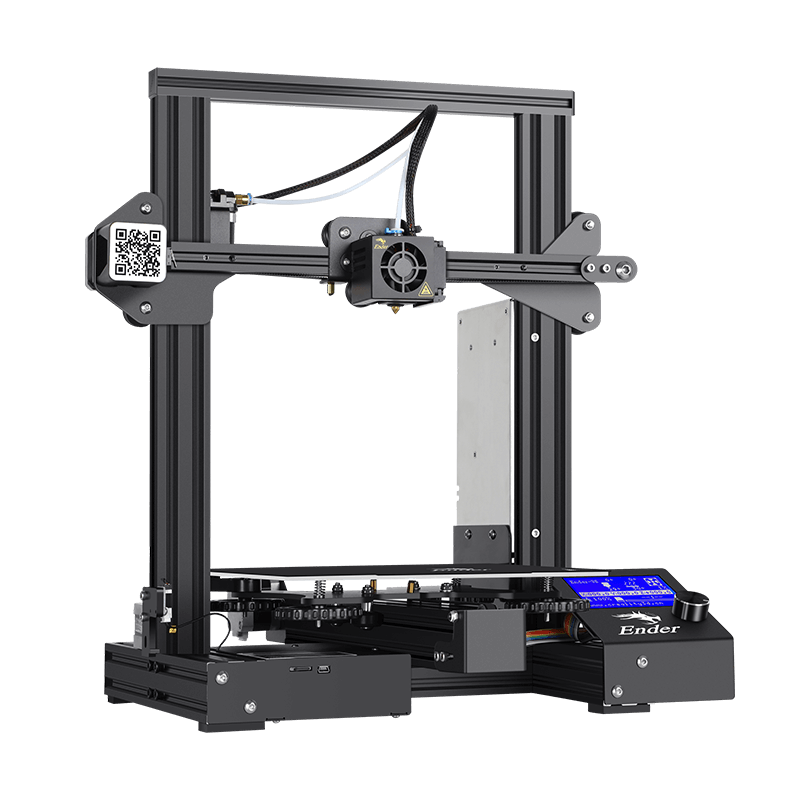
\includegraphics[width=\linewidth]{ender3}
  \ccaption{Ender 3 FDM-Drucker}{\url{https://3dee.at/wp-content/uploads/2022/09/creality-ender-3-tiny.png}}
  \label{img:fdm}
\end{minipage}%
\begin{minipage}{.5\textwidth}
  \centering
  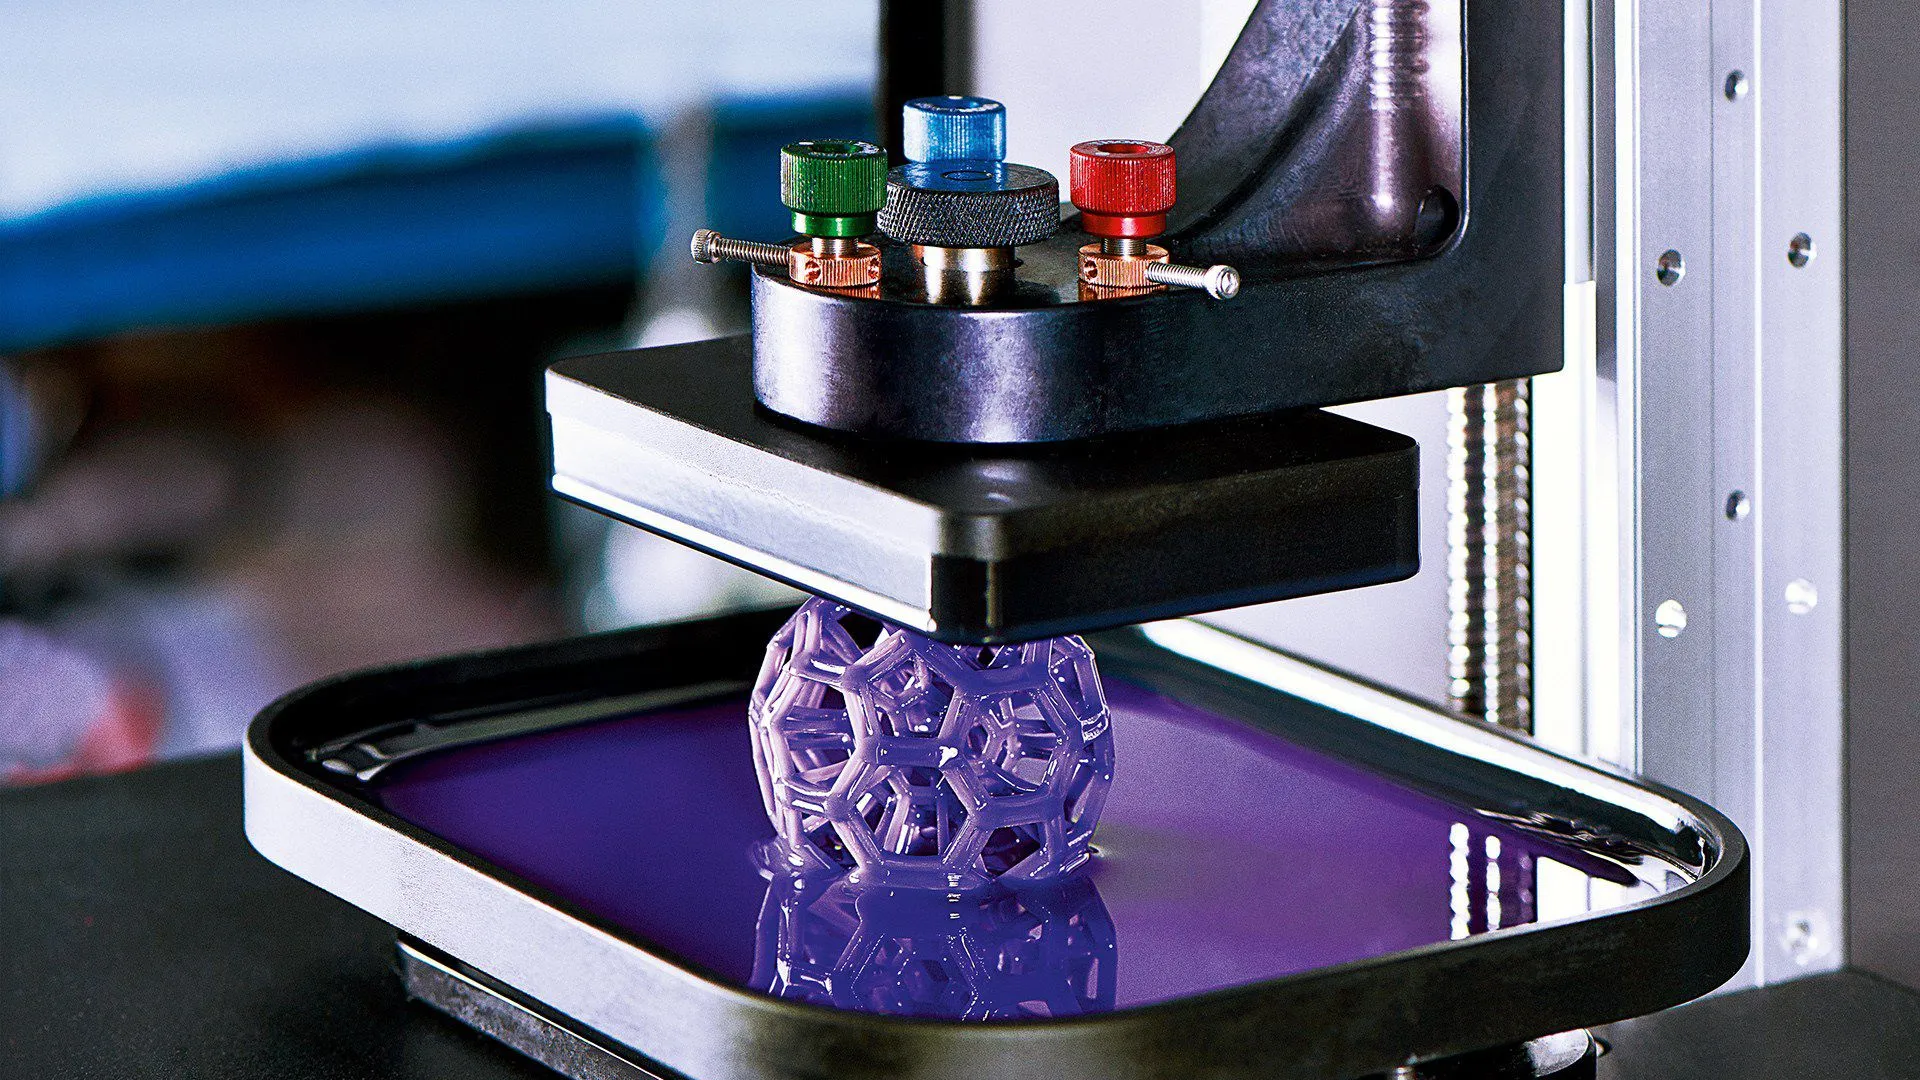
\includegraphics[width=\linewidth]{sla_printer}
  \ccaption{SLA-Drucker Aufbau}{\url{https://3dee.at/wp-content/uploads/2022/09/creality-ender-3-tiny.png}}
  \label{img:sla}
\end{minipage}
\end{figure}

Das erste Pulverbett-Metall-3D-Druck-Verfahren, \acrfull{slm}, wurde kurz darauf im Jahr 1995 in Deutschland entwickelt und patentiert. Es wird unter vielen Namen vertrieben, wie \it{Direct Metal Laser Sintering} oder unter dem Überbegriff \it{Powder-Bed-Fusion}. Offiziell wurde des Verfahren als Sinter-Verfahren eingestuft durch die IEEE (\it{Institute of Electrical and Electronics Engineers}), was jedoch eine wissenschaftlich gesehen falsche Kategorisierung ist, da ein Sinter-Verfahren das Grundmaterial nur \say{erweicht} und nicht vollständig aufschmilzt, wie es im SLM-Prozess geschieht. \parencite{SINTER_SMELT} Übliche Materialien für den SLM-Druck sind Aluminium-, Stahl- und Titan-Legierungen. Oft verwendet wird der Edelstahl 316L mit einem Schmelzpunkt von \qty{1390}{\celsius} und \qty{1440}{\degreeCelsius} \parencite{610LSTEEL} oder der Werkzeugstahl 1.2709 für Spritzguss-Formen. \parencite{steel12709} Diese Temperatur ist nur bewerkstelligbar durch einen starken Laser mit einer Leistung von \qty{400}{\watt} bis hin zu über \qty{12}{\kilo\watt}.
\subsection{Digitale Erschaffung und Darstellung}
Die Grundlage eines jeden 3D-gedruckten Modells ist ein \acrfull{cad}, welches das gewünschte Teil durch 2D-Zeichnungen darstellt, welche danach zu Körpern extrudiert werden mit verschiedenen Tools. Diese Modelle werden  in \it{Standard-Tesselation-Language} (STL) konvertiert. Ein solches \it{Mesh} ist in Abbildung \ref{img:stl_1} erkennbar anhand einer Kugel. Dieses Format ist für den \it{Slicer}, ein Programm, welches das Modell für den Drucker konvertiert gedacht. Ein Slicer (engl. \it{to slice}: schneiden), \say{schneidet} das Modell in Schichten, welche der Drucker dann auftragen kann. Zusätlich kontrolliert er zumeist die Einstellungen mit welchen der Drucker arbeitet (z.B. Temperatur, Schichtdicke, Geschwindigkeit, o.Ä.). Eine STL-Datei stellt das Modell als eine Punktwolke dar, wobei immer 3 Punkte ein Dreieck, auch bekannt als \it{Facet} oder \it{Face}, bilden. Ein weiterer Aspekt, welcher von STL-Dateien gespeichert wird ist der Normalvektor eines jeden Dreiecks, mit welchem der Slicer berechnen kann, ob es eine \say{innere} oder \say{äußere} Wand ist, um eine etwaige Füllung des Teils mit \it{Lattice}-Strukturen, also einem unterstützenden Gerüst, zu ermöglichen ohne das äußere Erscheinungsbild zu beeinträchtigen. Dies ist insofern relevant, da schlecht exportierte STL-Dateien oft fehlerhafte Normalvektoren enthalten und somit beinahe undruckbar sind ohne manuelle Reperatur durch Rückführung in die originale Topologie, welche rechnerisch sehr aufwendig ist und nicht ohne Detailverluste möglich ist.
\begin{figure}[h]
\begin{center}
	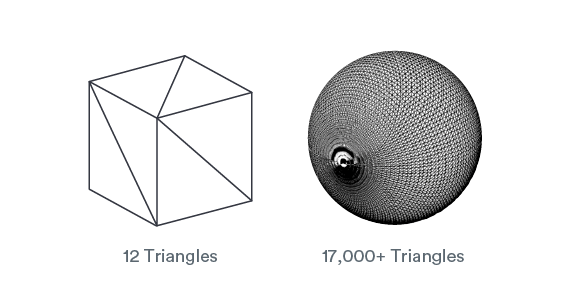
\includegraphics[width=.7\textwidth]{stl_file_1}
	\ccaption{Wireframe eines Würfels und einer Kugel im STL-Datenformat}{\url{https://www.protolabs.com/media/1022944/pl-dt-may-2021_570x308-02.png}}
	\label{img:stl_1}
\end{center}
\end{figure}	
Das STL-Format ist sehr effizient darin, ebene Oberflächen darzustellen, da diese aus mehreren Dreiecken bestehen. Wenn jedoch eine Krümmung einzurechnen ist, muss wie in Abb. \ref{img:stl_1} zu erkennen ist, diese Krümmung mit Dreiecken angenähert werden. Dieser Vorgang führt eine Ungenauigkeit ein, welche durch Approxmiationen eingedämmt werden kann. Daraus können oft Dateien im Gigabyte-Bereich entstehen, welche mit Optimierung nur einige Megabyte groß sein würden. Zu große Dateien können bei Druckern mit begrenztem Arbeitsspeicher zu einem Absturz während des Drucks führen und dabei sogar die Maschine beschädigen. \parencite{stl_1} 

Als Alternative zum STL-Format steht das STEP-Format, welches Krümmungen mit sogenannten \it{Non-Uniform Rational B-Splines (NURBS)} darstellt.
Diese ermöglichen es, beliebige Kurven und Formen darzustellen. Das Format wird immer beliebter, wobei es noch weit vom Nutzungsgrad der STL-Dateien entfernt ist, da es rechnerisch intensiver ist und von vielen populären Programmen nicht unterstützt wird die im Hobby- \& Industriebereich verwendet werden. Die Präzision dieses Formats ist oft hoch gelobt, jedoch in der Praxis aufgrund von schlecht kalibrierten Maschinen sowie auch technischen Limitationen in den meisten Fällen nicht relevant. \parencite{ADOBESTEP}
\end{document}
